% !TEX TS-program = pdflatex
% !TEX encoding = UTF-8 Unicode

\documentclass{beamer}
% for handouts: \documentclass[handout]{beamer}

%\setbeamertemplate{background canvas}[vertical shading][bottom=white,top=structure.fg!25]
% or whatever

\usetheme[compress]{Amsterdam}
%\setbeamertemplate{headline}{}
%\setbeamertemplate{footline}{}
%\setbeamersize{text margin left=0.5cm}
  
\usepackage[english]{babel}
\usepackage{listings}
\usepackage{geometry}
\usepackage{hyperref}
\usepackage{multicol}


\usepackage[utf8]{inputenc}
\usepackage[T1]{fontenc}
\usepackage{lmodern}

\lstset{
basicstyle=\scriptsize\ttfamily,
columns=flexible,
breaklines=true,
numbers=left,
%stepsize=1,
numberstyle=\tiny,
backgroundcolor=\color[rgb]{0.85,0.90,1}
}


\begin{document}


\title[Big Data and Automated Content Analysis]{\textbf{Big Data and Automated Content Analysis} \\ Week 5 -- Tuesday \\ Automated content analysis with NLP and regular expressions}
\author[Damian Trilling]{Damian Trilling \\ ~ \\ \footnotesize{d.c.trilling@uva.nl \\@damian0604} \\ \url{www.damiantrilling.net}}
\date{28 April 2020}
\institute[UvA]{Afdeling Communicatiewetenschap \\Universiteit van Amsterdam}

%\maketitle
\begin{frame}[plain]{}
\titlepage
\end{frame}

\begin{frame}{Today}
\tableofcontents
\end{frame}

%{\setbeamercolor{background canvas}{bg=black}
%\begin{frame}[plain]
%\makebox[\linewidth]{
%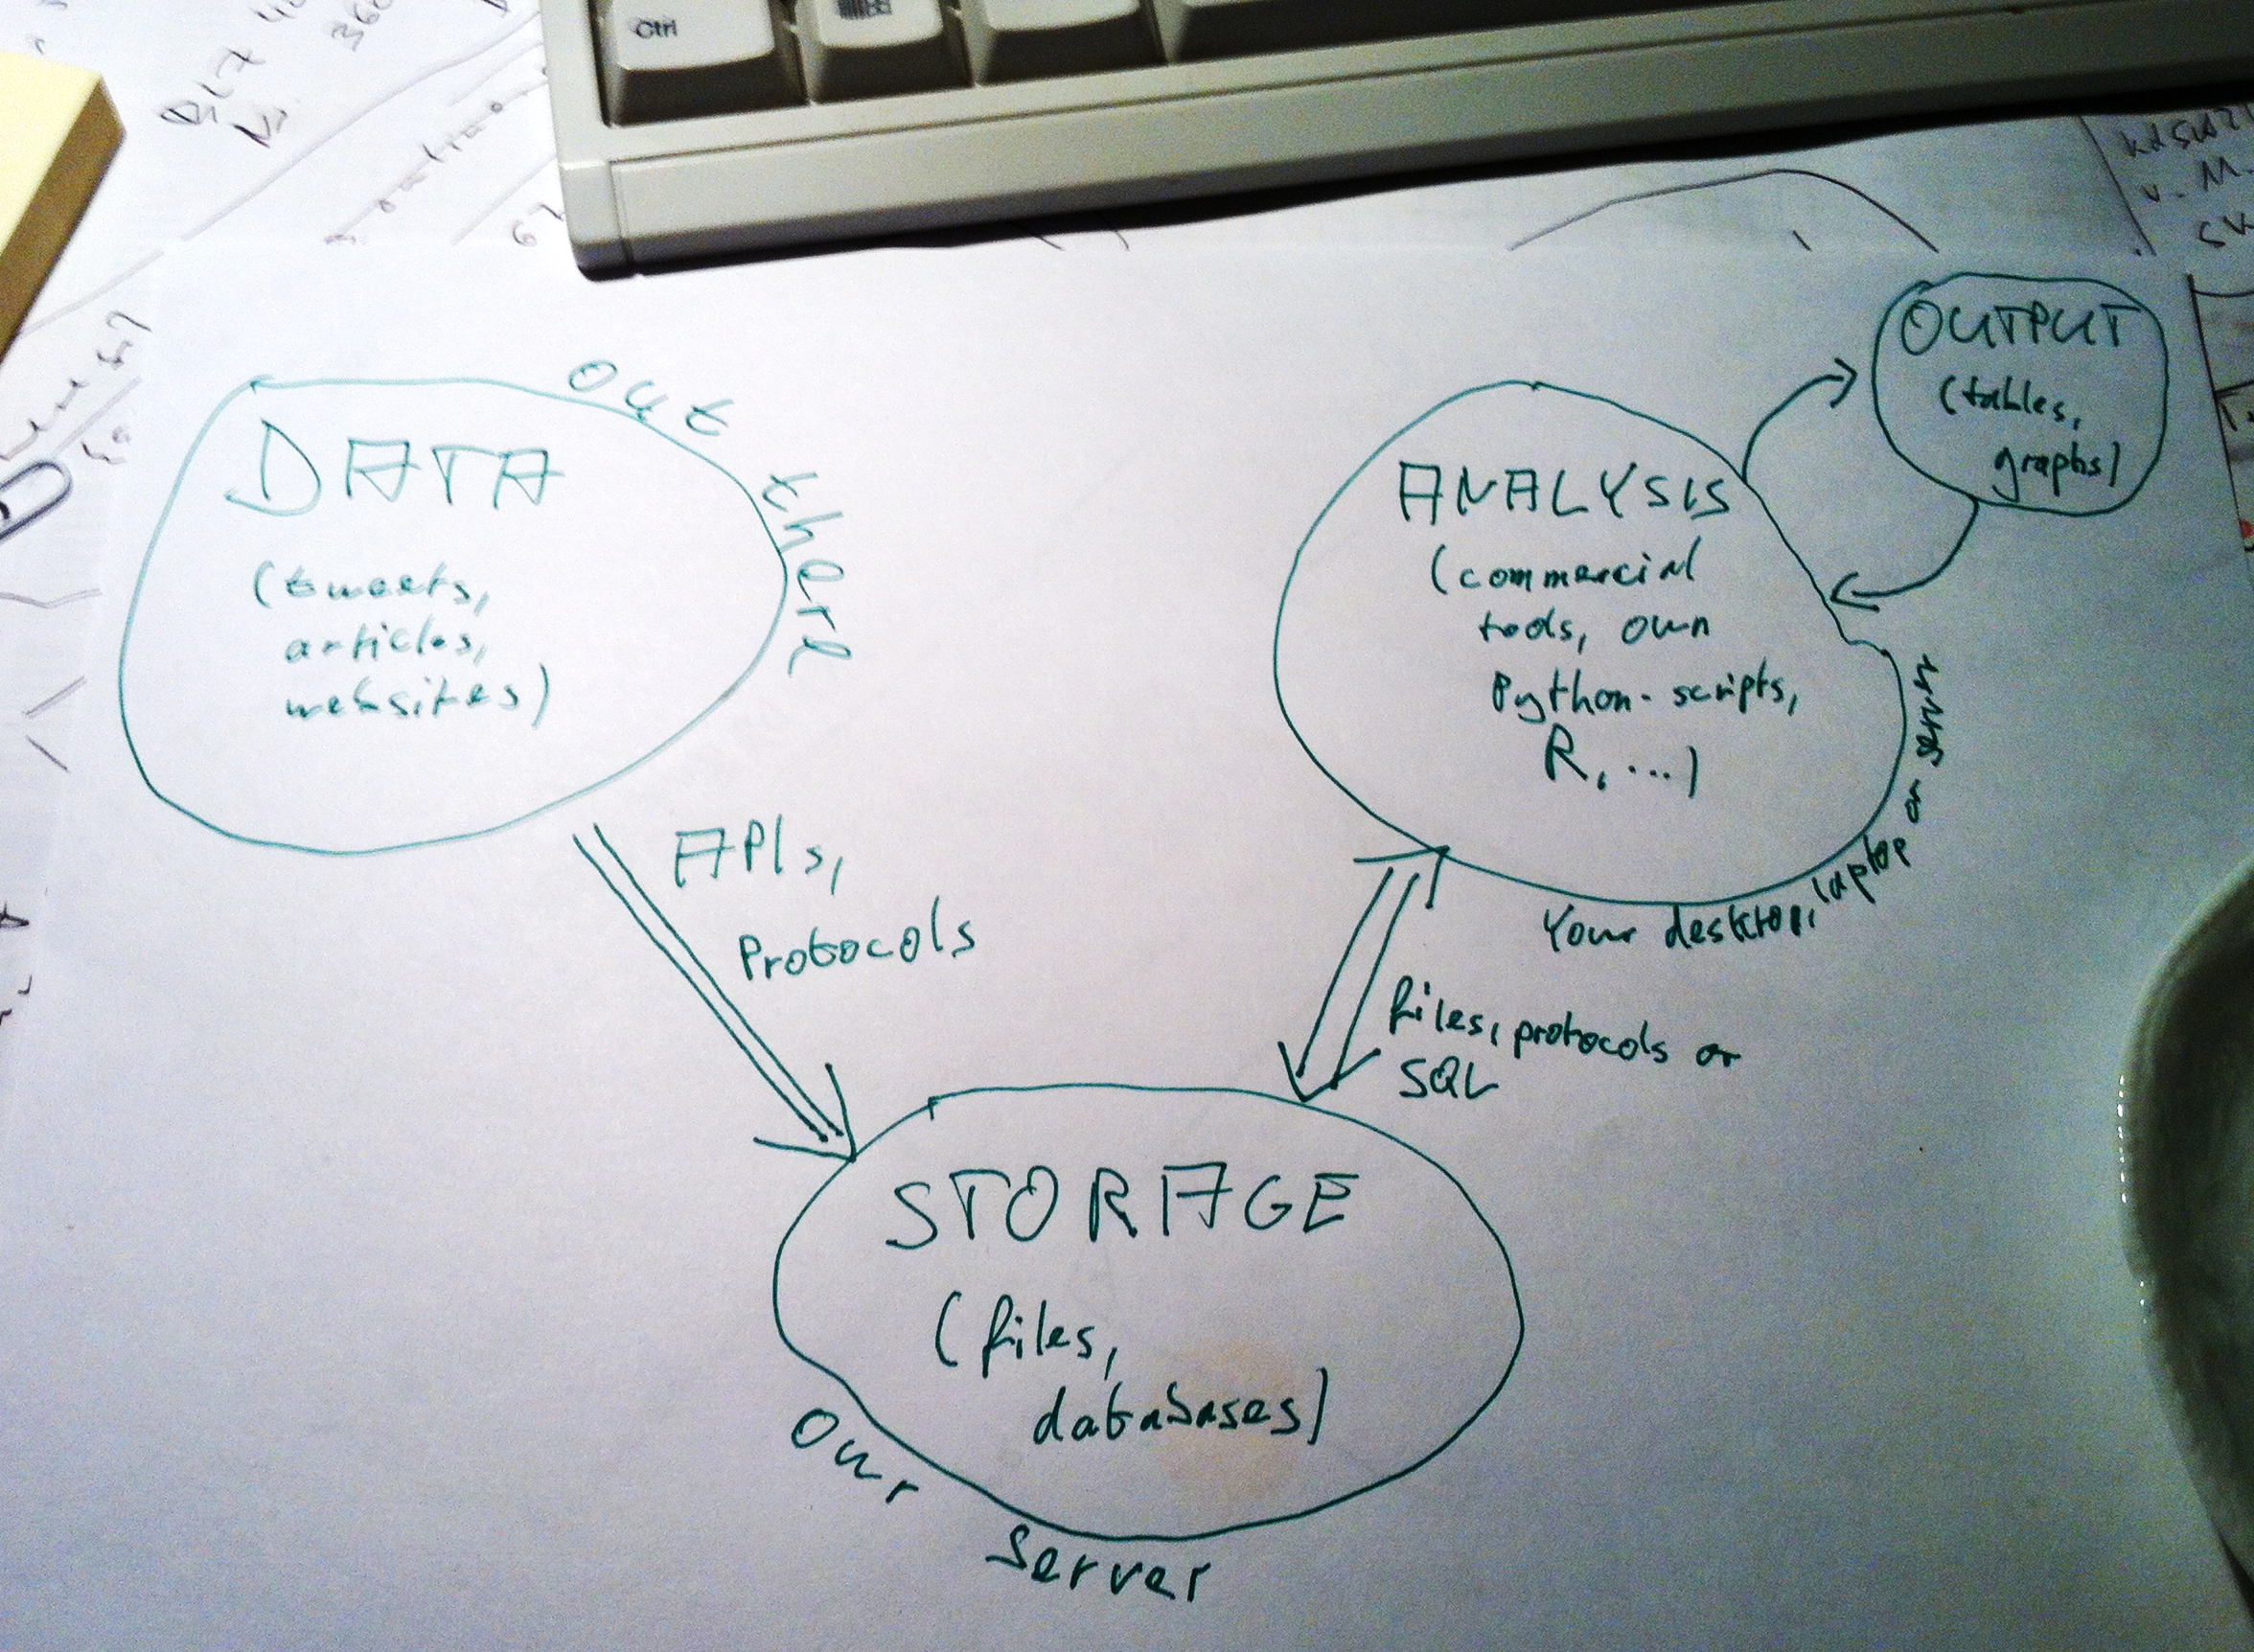
\includegraphics[width=\paperwidth,height=\paperheight,keepaspectratio]{process-heel.png}}
%\end{frame}
%}


\section[Regular expressions]{ACA using regular expressions}

\begin{frame}
Automated content analysis using regular expressions
\end{frame}


\subsection{Bottom-up vs. top-down}

\begin{frame}{Bottom-up vs. top-down}
	\begin{block}{Bottom-up}
	\begin{itemize}
		\item Count most frequently occurring words (Week 2)
		\item Maybe better: Count combinations of words $\Rightarrow$ Which words co-occur together? (Chapter 9, not obligatory)
	\end{itemize}
	We \emph{don't} specify what to look for in advance	
	\end{block}
	
	\onslide<2>{
	\begin{block}{Top-down}
	\begin{itemize}
		\item Count frequencies of pre-defined words (like in BOW-sentiment analysis)
		\item Maybe better: patterns instead of words (\textbf{regular expressions, today!})
	\end{itemize}
	We \emph{do} specify what to look for in advance	
\end{block}
}
%\tiny{see also Boumans \& Trilling (2016)}
\end{frame}




\subsection{What is a regexp?}
\begin{frame}{Regular Expressions: What and why?}
\begin{block}{What is a regexp?}
\begin{itemize}
\item<1-> a \emph{very} widespread way to describe patterns in strings
\item<2-> Think of wildcards like {\tt{*}} or operators like {\tt{OR}}, {\tt{AND}} or {\tt{NOT}} in search strings: a regexp does the same, but is \emph{much} more powerful
\item<3-> You can use them in many editors (!), in the Terminal, in STATA \ldots and in Python
\end{itemize}
\end{block}
\end{frame}

\begin{frame}{An example}
\begin{block}{From last week's task}
\begin{itemize}
\item We wanted to remove everything but words from a tweet
\item We did so by calling the \texttt{.replace()} method
\item We could do this with a regular expression as well: \\
{\tt{ \lbrack \^{}a-zA-Z\rbrack}} would match anything that is not a letter
\end{itemize}
\end{block}
\end{frame}

\begin{frame}{Basic regexp elements}
\begin{block}{Alternatives}
\begin{description}
\item[{\tt{\lbrack TtFf\rbrack}}] matches either T or t or F or f
\item[{\tt{Twitter|Facebook}}] matches either Twitter or Facebook
\item[{\tt{.}}] matches any character
\end{description}
\end{block}
\begin{block}{Repetition}<2->
\begin{description}
\item[{\tt{*}}] the expression before occurs 0 or more times
\item[{\tt{+}}] the expression before occurs 1 or more times
\end{description}
\end{block}
\end{frame}

\begin{frame}{regexp quizz}
\begin{block}{Which words would be matched?}
\tt
\begin{enumerate}
\item<1-> \lbrack Pp\rbrack ython
\item<2-> \lbrack A-Z\rbrack +
\item<3-> RT ?:? @\lbrack a-zA-Z0-9\rbrack +
\end{enumerate}
\end{block}
\end{frame}

\begin{frame}{What else is possible?}
If you google {\tt{regexp}} or {\tt{regular expression}}, you'll get a bunch of useful overviews. The wikipedia page is not too bad, either. 
\end{frame}

\subsection{Using a regexp in Python}
\begin{frame}{How to use regular expressions in Python}
\begin{block}{The module re}
\begin{description}
\item<1->[{\tt{re.findall("\lbrack Tt\rbrack witter|\lbrack Ff\rbrack acebook",testo)}}] returns a list with all occurances of Twitter or Facebook in the string called {\tt{testo}}
\item<1->[{\tt{re.findall("\lbrack 0-9\rbrack +\lbrack a-zA-Z\rbrack +",testo)}}] returns a list with all words that start with one or more numbers followed by one or more letters in the string called {\tt{testo}}
\item<2->[{\tt{re.sub("\lbrack Tt\rbrack witter|\lbrack Ff\rbrack acebook","a social medium",testo)}}] returns a string in which all all occurances of Twitter or Facebook are replaced by "a social medium"
\end{description}
\end{block}
\end{frame}


\begin{frame}[fragile]{How to use regular expressions in Python}
\begin{block}{The module re}
\begin{description}
\item<1->[{\tt{re.match(" +(\lbrack 0-9\rbrack +) of (\lbrack 0-9\rbrack +) points",line)}}] returns  \texttt{None} unless it \emph{exactly} matches the string \texttt{line}. If it does, you can access the part between () with the \texttt{.group()} method.
\end{description}
\end{block}

Example:
\begin{lstlisting}
line="             2 of 25 points"
result=re.match(" +([0-9]+) of ([0-9]+) points",line)
if result:
   print ("Your points:",result.group(1))
   print ("Maximum points:",result.group(2))
\end{lstlisting}
Your points: 2\\
Maximum points: 25
\end{frame}














\begin{frame}{Possible applications}
\begin{block}{Data preprocessing}
\begin{itemize}
\item Remove unwanted characters, words, \ldots
\item Identify \emph{meaningful} bits of text: usernames, headlines, where an article starts, \ldots
\item filter (distinguish relevant from irrelevant cases)
\end{itemize}
\end{block}
\end{frame}


\begin{frame}{Possible applications}
\begin{block}{Data analysis: Automated coding}
\begin{itemize}
\item Actors
\item Brands
\item links or other markers that follow a regular pattern
\item Numbers (!)
\end{itemize}
\end{block}
\end{frame}

\begin{frame}[fragile,plain]{Example 1: Counting actors}
\begin{lstlisting}
import re, csv
from glob import glob
count1_list=[]
count2_list=[]
filename_list = glob("/home/damian/articles/*.txt")

for fn in filename_list:
   with open(fn) as fi:
      artikel = fi.read()
      artikel = artikel.replace('\n',' ')
      
      count1 = len(re.findall('Israel.*(minister|politician.*|[Aa]uthorit)',artikel))
      count2 = len(re.findall('[Pp]alest',artikel))

      count1_list.append(count1)
      count2_list.append(count2)
      
output=zip(filename_list,count1_list, count2_list)
with open("results.csv", mode='w',encoding="utf-8") as fo:
    writer = csv.writer(fo)
    writer.writerows(output)
\end{lstlisting}
\end{frame}




\begin{frame}[fragile]{Example 2: Which number has this Lexis Nexis article?}
\begin{lstlisting}
                              All Rights Reserved

                               2 of 200 DOCUMENTS

                                  De Telegraaf

                             21 maart 2014 vrijdag

Brussel bereikt akkoord  aanpak probleembanken;
ECB krijgt meer in melk te brokkelen

SECTION: Finance; Blz. 24
LENGTH: 660 woorden

BRUSSEL   Europa heeft gisteren op de valreep een akkoord bereikt 
over een saneringsfonds voor banken. Daarmee staat de laatste
\end{lstlisting}

\end{frame}

\begin{frame}[fragile]{Example 2: Check the number of a lexis nexis article}
\begin{lstlisting}
                              All Rights Reserved

                               2 of 200 DOCUMENTS

                                  De Telegraaf

                             21 maart 2014 vrijdag

Brussel bereikt akkoord  aanpak probleembanken;
ECB krijgt meer in melk te brokkelen

SECTION: Finance; Blz. 24
LENGTH: 660 woorden

BRUSSEL   Europa heeft gisteren op de valreep een akkoord bereikt 
over een saneringsfonds voor banken. Daarmee staat de laatste
\end{lstlisting}

\begin{lstlisting}
for line in tekst:
    matchObj=re.match(r" +([0-9]+) of ([0-9]+) DOCUMENTS",line)
    if matchObj:
        numberofarticle= int(matchObj.group(1))
        totalnumberofarticles= int(matchObj.group(2))
\end{lstlisting}
\end{frame}


\begin{frame}{Practice yourself!}
\huge{\url{http://www.pyregex.com/}}
\end{frame}



\section{Natural Language Processing}
\begin{frame}
Natural Language Processing
\end{frame}



\begin{frame}{NLP: What and why?}
\begin{block}{What can we do?}
\begin{itemize}
\item<1-> remove stopwords
\item<2-> stemming
\item<3-> parse sentences (advanced)
\end{itemize}
\end{block}
\end{frame}






\subsection{Stopword removal}
\begin{frame}
	Natural Language Processing:\\
	\textbf{Stopword removal} \\
	\vspace{1cm}
	\onslide<2>{\emph{Have a look back at last week! The logic of the algorithm is very much related to the one of our first simple sentiment analysis!}}
\end{frame}


\begin{frame}{Stopword removal: What and why?}
	\begin{block}{Why remove stopwords?}
		\begin{itemize}
			\item If we want to identify key terms (e.g., by means of a word count), we are not interested in them
			\item If we want to calculate document similarity, it might be inflated
			\item If we want to make a word co-occurance graph, irrelevant information will dominate the picture
		\end{itemize}
	\end{block}
\end{frame}


\begin{frame}[fragile]{Stopword removal: How}
\begin{lstlisting}
testo='He gives her a beer and a cigarette.'
testonuovo=""
stopwords=['and','the','a','or','he','she','him','her']
for verbo in testo.split():
    if verbo not in stopwords:
        testonuovo=testonuovo+verbo+" "
\end{lstlisting}
What do we get if we do:
\begin{lstlisting}
print (testonuovo)
\end{lstlisting}
Can you explain the algorithm?
\end{frame}

\begin{frame}[fragile]{We get:}
\begin{lstlisting}
>>> print  (testonuovo)
'He gives beer cigarette. '
\end{lstlisting}
Why is "He" still in there? \\ How can we fix this?
\end{frame}

\begin{frame}[fragile]{Stopword removal}
\begin{lstlisting}
testo='He gives her a beer and a cigarette.'
testonuovo=""
stopwords=['and','the','a','or','he','she','him','her']
for verbo in testo.split():
    if verbo.lower() not in stopwords:
        testonuovo=testonuovo+verbo+" "
\end{lstlisting}
\end{frame}












\subsection{Stemming}
\begin{frame}{NLP: What and why?}
\begin{block}{Why do stemming?}
\begin{itemize}
\item Because we do not want to distinguish between smoke, smoked, smoking, \ldots
\item Typical preprocessing step (like stopword removal)
\end{itemize}
\end{block}
\end{frame}









\begin{frame}[fragile]{Stemming}
{\footnotesize{(with NLTK, see Bird, S., Loper, E., \& Klein, E. (2009). \emph{Natural language processing with Python}. Sebastopol, CA: O’Reilly.)}}
\begin{lstlisting}
from nltk.stem.snowball import SnowballStemmer
stemmer=SnowballStemmer("english")
frase="I am running while generously greeting my neighbors"
frasenuevo=""
for palabra in frase.split():
    frasenuevo=frasenuevo + stemmer.stem(palabra)  + " "
\end{lstlisting}
If we now did {\tt{print(frasenuevo)}}, it would return:
\begin{lstlisting}
i am run while generous greet my neighbor
\end{lstlisting}
\end{frame}

\begin{frame}[fragile]{Stemming and stopword removal - let's combine them!}
\begin{lstlisting}
from nltk.stem.snowball import SnowballStemmer
from nltk.corpus import stopwords
stemmer=SnowballStemmer("english")
mystopwords = stopwords.words("english")
frase="I am running while generously greeting my neighbors"
frasenuevo=""
for palabra in frase.lower().split():
    if palabra not in mystopwords:
        frasenuevo=frasenuevo + stemmer.stem(palabra)  + " "
\end{lstlisting}
Now, {\tt{print(frasenuevo)}} returns:
\begin{lstlisting}
run generous greet neighbor
\end{lstlisting}
Perfect!\\
\onslide<2>{
\tiny{In order to use \texttt{nltk.corpus.stopwords}, you have to download that module once. You can do so by typing the following in the Python console and selecting the appropriate package from the menu that pops up: \\ \texttt{import nltk\\nltk.download()}\\NB: Don't download everything, that's several GB.\\}}
\end{frame}

{\setbeamercolor{background canvas}{bg=black}
\begin{frame}[plain]
\makebox[\linewidth]{
\includegraphics[width=\paperwidth,height=\paperheight,keepaspectratio]{../../pictures/nltk-download.png}}
\end{frame}
}



\subsection{Parsing sentences}
\begin{frame}{NLP: What and why?}
\begin{block}{Why parse sentences?}
\begin{itemize}
\item To find out what grammatical function words have
\item and to get closer to the meaning.
\end{itemize}
\end{block}
\end{frame}

\begin{frame}[fragile]{Parsing a sentence}
\begin{lstlisting}
import nltk
sentence = "At eight o'clock on Thursday morning, Arthur didn't feel very good."
tokens = nltk.word_tokenize(sentence)
print (tokens)
\end{lstlisting}

\texttt{nltk.word\_tokenize(sentence)} is similar to sentence.split(), but compare handling of punctuation and the \texttt{didn't} in the output:
\begin{lstlisting}
['At', 'eight', "o'clock", 'on', 'Thursday', 'morning','Arthur', 'did', "n't", 'feel', 'very', 'good', '.']
\end{lstlisting}
\end{frame}


\begin{frame}[fragile]{Parsing a sentence}
Now, as the next step, you can ``tag'' the tokenized sentence:
\begin{lstlisting}
tagged = nltk.pos_tag(tokens)
print (tagged[0:6])
\end{lstlisting}
gives you the following:
\begin{lstlisting}
[('At', 'IN'), ('eight', 'CD'), ("o'clock", 'JJ'), ('on', 'IN'),
('Thursday', 'NNP'), ('morning', 'NN')]
\end{lstlisting}

\onslide<2->{
And you could get the word type of "morning" with \texttt{tagged[5][1]}!
}

\end{frame}


\begin{frame}{More NLP}
  \Huge{Look at \url{http://nltk.org}}

  \Huge{Look at \url{http://spacy.io}}

  \Huge{Look at \url{https://stanfordnlp.github.io/stanza/}}



\end{frame}




\section{Next steps}

\begin{frame}[plain]
\huge Next steps
  \end{frame}


\begin{frame}{Take-home messages}
\begin{block}{What you should be familiar with:}
\begin{itemize}
\item Possible steps to preprocess the data
\item Regular expressions
\item Word counts
\end{itemize}
\end{block}
\end{frame}





\begin{frame}{Thursday meeting}

  \begin{block}{Exercise}
    Exercise: 
    \url{https://github.com/damian0604/bdaca/blob/master/rm-course-1/week5/regexp-exercise.txt}

    \begin{itemize}
    \item Make some test strings
    \item Check wether your regex works as expected
    \end{itemize}


  \end{block}
  
\begin{block}{Two options for Thursday:}
\begin{itemize}
\item If there are many questions on Canvas: We'll discuss them.
\item If not: I'll already introduce you to statistics in Python (week 7) so that we can do cooler stuff in week 7 (like topic modelling)
\end{itemize}
\end{block}
\end{frame}



\end{document}


